% Options for packages loaded elsewhere
\PassOptionsToPackage{unicode}{hyperref}
\PassOptionsToPackage{hyphens}{url}
\PassOptionsToPackage{dvipsnames,svgnames,x11names}{xcolor}
%
\documentclass[
  letterpaper,
  DIV=11,
  numbers=noendperiod]{scrartcl}

\usepackage{amsmath,amssymb}
\usepackage{iftex}
\ifPDFTeX
  \usepackage[T1]{fontenc}
  \usepackage[utf8]{inputenc}
  \usepackage{textcomp} % provide euro and other symbols
\else % if luatex or xetex
  \usepackage{unicode-math}
  \defaultfontfeatures{Scale=MatchLowercase}
  \defaultfontfeatures[\rmfamily]{Ligatures=TeX,Scale=1}
\fi
\usepackage{lmodern}
\ifPDFTeX\else  
    % xetex/luatex font selection
\fi
% Use upquote if available, for straight quotes in verbatim environments
\IfFileExists{upquote.sty}{\usepackage{upquote}}{}
\IfFileExists{microtype.sty}{% use microtype if available
  \usepackage[]{microtype}
  \UseMicrotypeSet[protrusion]{basicmath} % disable protrusion for tt fonts
}{}
\makeatletter
\@ifundefined{KOMAClassName}{% if non-KOMA class
  \IfFileExists{parskip.sty}{%
    \usepackage{parskip}
  }{% else
    \setlength{\parindent}{0pt}
    \setlength{\parskip}{6pt plus 2pt minus 1pt}}
}{% if KOMA class
  \KOMAoptions{parskip=half}}
\makeatother
\usepackage{xcolor}
\ifLuaTeX
  \usepackage{luacolor}
  \usepackage[soul]{lua-ul}
\else
  \usepackage{soul}
  
\fi
\setlength{\emergencystretch}{3em} % prevent overfull lines
\setcounter{secnumdepth}{5}
% Make \paragraph and \subparagraph free-standing
\makeatletter
\ifx\paragraph\undefined\else
  \let\oldparagraph\paragraph
  \renewcommand{\paragraph}{
    \@ifstar
      \xxxParagraphStar
      \xxxParagraphNoStar
  }
  \newcommand{\xxxParagraphStar}[1]{\oldparagraph*{#1}\mbox{}}
  \newcommand{\xxxParagraphNoStar}[1]{\oldparagraph{#1}\mbox{}}
\fi
\ifx\subparagraph\undefined\else
  \let\oldsubparagraph\subparagraph
  \renewcommand{\subparagraph}{
    \@ifstar
      \xxxSubParagraphStar
      \xxxSubParagraphNoStar
  }
  \newcommand{\xxxSubParagraphStar}[1]{\oldsubparagraph*{#1}\mbox{}}
  \newcommand{\xxxSubParagraphNoStar}[1]{\oldsubparagraph{#1}\mbox{}}
\fi
\makeatother


\providecommand{\tightlist}{%
  \setlength{\itemsep}{0pt}\setlength{\parskip}{0pt}}\usepackage{longtable,booktabs,array}
\usepackage{calc} % for calculating minipage widths
% Correct order of tables after \paragraph or \subparagraph
\usepackage{etoolbox}
\makeatletter
\patchcmd\longtable{\par}{\if@noskipsec\mbox{}\fi\par}{}{}
\makeatother
% Allow footnotes in longtable head/foot
\IfFileExists{footnotehyper.sty}{\usepackage{footnotehyper}}{\usepackage{footnote}}
\makesavenoteenv{longtable}
\usepackage{graphicx}
\makeatletter
\def\maxwidth{\ifdim\Gin@nat@width>\linewidth\linewidth\else\Gin@nat@width\fi}
\def\maxheight{\ifdim\Gin@nat@height>\textheight\textheight\else\Gin@nat@height\fi}
\makeatother
% Scale images if necessary, so that they will not overflow the page
% margins by default, and it is still possible to overwrite the defaults
% using explicit options in \includegraphics[width, height, ...]{}
\setkeys{Gin}{width=\maxwidth,height=\maxheight,keepaspectratio}
% Set default figure placement to htbp
\makeatletter
\def\fps@figure{htbp}
\makeatother
% definitions for citeproc citations
\NewDocumentCommand\citeproctext{}{}
\NewDocumentCommand\citeproc{mm}{%
  \begingroup\def\citeproctext{#2}\cite{#1}\endgroup}
\makeatletter
 % allow citations to break across lines
 \let\@cite@ofmt\@firstofone
 % avoid brackets around text for \cite:
 \def\@biblabel#1{}
 \def\@cite#1#2{{#1\if@tempswa , #2\fi}}
\makeatother
\newlength{\cslhangindent}
\setlength{\cslhangindent}{1.5em}
\newlength{\csllabelwidth}
\setlength{\csllabelwidth}{3em}
\newenvironment{CSLReferences}[2] % #1 hanging-indent, #2 entry-spacing
 {\begin{list}{}{%
  \setlength{\itemindent}{0pt}
  \setlength{\leftmargin}{0pt}
  \setlength{\parsep}{0pt}
  % turn on hanging indent if param 1 is 1
  \ifodd #1
   \setlength{\leftmargin}{\cslhangindent}
   \setlength{\itemindent}{-1\cslhangindent}
  \fi
  % set entry spacing
  \setlength{\itemsep}{#2\baselineskip}}}
 {\end{list}}
\usepackage{calc}
\newcommand{\CSLBlock}[1]{\hfill\break\parbox[t]{\linewidth}{\strut\ignorespaces#1\strut}}
\newcommand{\CSLLeftMargin}[1]{\parbox[t]{\csllabelwidth}{\strut#1\strut}}
\newcommand{\CSLRightInline}[1]{\parbox[t]{\linewidth - \csllabelwidth}{\strut#1\strut}}
\newcommand{\CSLIndent}[1]{\hspace{\cslhangindent}#1}

\KOMAoption{captions}{tableheading}
\makeatletter
\@ifpackageloaded{caption}{}{\usepackage{caption}}
\AtBeginDocument{%
\ifdefined\contentsname
  \renewcommand*\contentsname{Table of contents}
\else
  \newcommand\contentsname{Table of contents}
\fi
\ifdefined\listfigurename
  \renewcommand*\listfigurename{List of Figures}
\else
  \newcommand\listfigurename{List of Figures}
\fi
\ifdefined\listtablename
  \renewcommand*\listtablename{List of Tables}
\else
  \newcommand\listtablename{List of Tables}
\fi
\ifdefined\figurename
  \renewcommand*\figurename{Figure}
\else
  \newcommand\figurename{Figure}
\fi
\ifdefined\tablename
  \renewcommand*\tablename{Table}
\else
  \newcommand\tablename{Table}
\fi
}
\@ifpackageloaded{float}{}{\usepackage{float}}
\floatstyle{ruled}
\@ifundefined{c@chapter}{\newfloat{codelisting}{h}{lop}}{\newfloat{codelisting}{h}{lop}[chapter]}
\floatname{codelisting}{Listing}
\newcommand*\listoflistings{\listof{codelisting}{List of Listings}}
\makeatother
\makeatletter
\makeatother
\makeatletter
\@ifpackageloaded{caption}{}{\usepackage{caption}}
\@ifpackageloaded{subcaption}{}{\usepackage{subcaption}}
\makeatother

\ifLuaTeX
  \usepackage{selnolig}  % disable illegal ligatures
\fi
\usepackage{bookmark}

\IfFileExists{xurl.sty}{\usepackage{xurl}}{} % add URL line breaks if available
\urlstyle{same} % disable monospaced font for URLs
\hypersetup{
  pdftitle={Accessing Homelessness Through the Lens of Homeless Shelters Across the Greater Toronto Area},
  pdfauthor={Chris Yong Hong Sen},
  colorlinks=true,
  linkcolor={blue},
  filecolor={Maroon},
  citecolor={Blue},
  urlcolor={Blue},
  pdfcreator={LaTeX via pandoc}}


\title{Accessing Homelessness Through the Lens of Homeless Shelters
Across the Greater Toronto Area}
\author{Chris Yong Hong Sen}
\date{September 24, 2024}

\begin{document}
\maketitle
\begin{abstract}
Increasing numbers of homeless shelter's overnight stay across different
regions of the Greater Toronto Area suggests an increasing need to focus
on homelessness and the efficacy of existing policies. Regions
experiencing greater increases in overnight stays between 2021 and 2023
have to be scrutinised even further in order for canada to reduce
incidences of homelessness.
\end{abstract}


\section{Introduction}\label{introduction}

Homelessness has been an ongoing issue in Canada. Since April 1, 2019,
the Government of Canada (2023) has began the initiative `Reaching Home:
Canada's Homelessness Strategy', aiming to reduce chronic homelessness
by 50\% before 2028. About \$6.2 billion have been funded to this
nationwide issue over the past 9 years. With a slew of policies
addressing different categories of homelessness, this paper aims to
analyse whether homelessness has improved since the approximate end of
COVID in 2021.

The remainder of this paper is structured as follows.
Section~\ref{sec-data} gives us insights about the dataset and the steps
used in obtaining the dataset. In Section~\ref{sec-conclusion}, we will
be validating the data with existing observations made across various
websources and performing our analysis of homelessness.

\newpage

\section{Data}\label{sec-data}

\subsection{\texorpdfstring{{Data
Attributes}}{Data Attributes}}\label{data-attributes}

The data provides us daily counts of homeless people served, categorised
by their demographics such as gender or age, as well as the type of
housing service available for homeless people. It also provides us
information about the number of beds and that are available and approved
for homeless individuals and families.

The original dataset contains over 43 different attributes\ldots{}

\begin{description}
\tightlist
\item[\_id:]
unique identifier.
\item[OCCUPANCY\_DATE:]
date of record collected at 4AM EDT the following day. eg. Jan 01, 2021
would be the data collected on Jan 02, 2021 4AM EDT.
\item[ORGANIZATION\_ID:]
unique ID identifying organisations that is robust to organisation name
changes.
\item[ORGANIZATION\_NAME:]
name of organisation offering overnight service.
\item[SHELTER\_ID:]
unique ID indentifying shelter groups that is robust to shelter name
changes.
\item[SHELTER\_GROUP:]
group for which the overnight program belongs to in Shelter Management
Information System (SMIS) database.
\item[LOCATION\_ID:]
unique ID identifying locations that is robust to location name changes.
\item[LOCATION\_NAME:]
name of location where overnight service is occuring.
\item[LOCATION\_ADDRESS:]
street address of the location of overnight service.
\item[LOCATION\_POSTAL\_CODE:]
postal code of location of overnight service.
\item[LOCATION\_CITY:]
city where overnight service is occuring.
\item[LOCATION\_PROVINCE:]
province where overnight service is occuring.
\item[PROGRAM\_ID:]
unique ID identifying overnight service programs that is robust to
program name changes.
\item[PROGRAM\_NAME:]
name of program.
\item[SECTOR:]
type of homeless shelter. Possible classifications includes, `adult
men', `adult women', `mixed adult' (co-ed or all gender), `youth' and
`family'.
\item[PROGRAM\_MODEL:]
classification of overnight service programs as either `Emergency' or
`Transitional'. Emergency refers to a program where any homeless people
has access to the program regardless of a valid referral. Transitional
refers to a specialised program catered to homeless individuals/families
with a valid referral.
\item[OVERNIGHT\_SERVICE\_TYPE:]
classification of the type of overnight service provided.
\end{description}

\begin{itemize}
\tightlist
\item
  Shelter - temporary accommodation and support services to facilitate
  the shift from homelessness to staying in a proper home
\item
  24-Hour Respite - an allied shelter service that emphasises greater
  and efficient accessibility to a safe shelter with necessities such as
  resting spaces, food, and service referrals.
\item
  Motel/Hotel - a program that provides beds/rooms through contracts
  with hotels, typically in response to emergencies.
\item
  Interim Housing - housing provided via contracts with apartment
  spaces.
\item
  Warming Centre - an allied shelter service that provides immediate
  housing for extreme cold weathers.
\item
  24-Hour Women's Drop-in - housing that is targeted to homeless women,
  transgender or gender-non-binary people.
\item
  Isolation/Recovery Site - dedicated COVID-19 site targetted at
  homeless people who contracted COVID-19.
\end{itemize}

\begin{description}
\tightlist
\item[PROGRAM\_AREA:]
classification on whether program is all year round or simply temporary
due to an unexpected emergency.
\item[SERVICE\_USER\_COUNT:]
a counter for homeless people/families using a particular overnight
service in a given day.
\item[CAPACITY\_TYPE:]
room-based or bed-based overnight service.
\item[CAPACITY\_ACTUAL\_BED:]
actual number of beds available during the overnight service.
\item[CAPACITY\_FUNDING\_BED:]
approved number of beds available for an overnight service.
\item[OCCUPIED\_BEDS:]
actual number of beds occupied by homeless people/families during an
overnight service.
\item[UNOCCUPIED\_BEDS:]
unoccupied beds calculated as CAPACITY\_ACTUAL\_BED minus OCCUPIED\_BED.
\item[UNAVAILABLE\_BEDS:]
beds that are unavailable for the program due to maintenance, outbreaks
or pest control, calculated as CAPACITY\_FUNDING\_BED minus
CAPACITY\_ACTUAL\_BED.
\item[CAPACITY\_ACTUAL\_ROOM:]
actual number of rooms available during the overnight service.
\item[CAPACITY\_FUNDING\_ROOM:]
approved number of rooms available for an overnight service.
\item[OCCUPIED\_ROOMS:]
actual number of rooms occupied by homeless people/families during an
overnight service.
\item[UNOCCUPIED\_ROOMS:]
unoccupied rooms calculated as CAPACITY\_ACTUAL\_ROOM minus
OCCUPIED\_ROOM.
\item[UNAVAILABLE\_ROOMS:]
rooms that are unavailable for the program due to maintenance, outbreaks
or pest control, calculated as CAPACITY\_FUNDING\_ROOM minus
CAPACITY\_ACTUAL\_ROOM.
\item[OCCUPANCY\_RATE\_BEDS:]
proportion of actual bed capacity occupied during a given overnight
service, calculated as OCCUPIED\_BED divided by CAPACITY\_ACTUAL\_BED.
\item[OCCUPANCY\_RATE\_ROOMS:]
proportion of actual room capacity occupied during a given overnight
service, calculated as OCCUPIED\_ROOM divided by CAPACITY\_ACTUAL\_ROOM.
\end{description}

\subsection{Data Collection}\label{data-collection}

Daily active overnight allied services and shelters data was collected
in the Shelter Management Information System (SMIS) database under the
division, Toronto Shelter and Support Services (TSSS). Prior to 2021,
TSSS has also collected data regarding homeless shelter counts. Since
then, the TSSS has revised the curation of the dataset. Major revisions
include\ldots{}

\begin{itemize}
\item
  \ul{Overnight Service Type}: Accounts for all overnight services
  instead of only those from shelter programs.
\item
  \ul{Capacity Type}: The new dataset distinguishes room based capacity
  and bed based capacity. This allows us to differentiate between
  homeless individuals and homeless families as room based capacity are
  geared towards households where the sleeping rooms are not shared by
  different families, while bed based capacity are characterised by a
  common and shared sleeping area. This prevents over reporting of the
  previous capacity of room based capacity.
\item
  \ul{Two Measures of Capacity}: The TSSS has since provided
  \textbf{Funding} capacity and \textbf{Actual} capacity. Funding
  capacity reports the \emph{intended} number of rooms/beds available
  for a particular day. Actual capacity reports the \emph{actual} number
  of rooms/beds provided for that day. Datasets prior to 2021 only
  included \textbf{Funding} capacity. Therefore, the \textbf{Actual}
  capacity would provide a more accurate representation of various
  program's overnight stay rates.
\end{itemize}

\section{Conclusion}\label{sec-conclusion}

\begin{figure}

\centering{

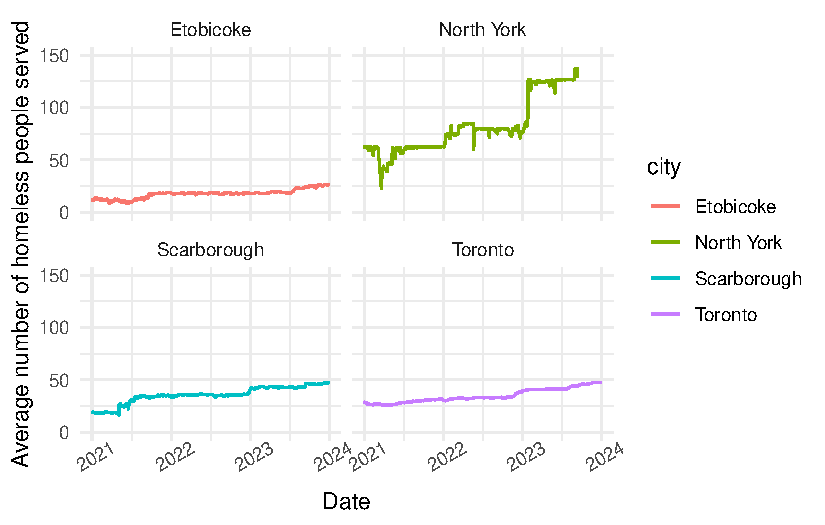
\includegraphics{paper_files/figure-pdf/fig-homelessness_across_cities-1.pdf}

}

\caption{\label{fig-homelessness_across_cities}number of homeless people
served from 2021 to 2023 across cities}

\end{figure}%

\subsection{Data Summary}\label{data-summary}

The situation provided by this dataset immediately alerts us to the city
of North York the number of homeless individuals/families serviced daily
has increased from beginning of 2021 to the end of 2023. Andrew
Palamarchuk North York Mirror (2023) posits that homeless shelters have
filled up only after 4 days of it's launch back in 2022. This simple
observation can be seen from Figure~\ref{fig-homelessness_across_cities}
under North York's scatter plot where there there were sporadic volatile
increases in the first quarter of 2022. Unfortunately, not much research
or journalism has been done to explore but the data presented by
\emph{About Daily Shelter \& Overnight Service Occupancy \& Capacity}
(2024) suggests that more can be done to help indiviuals and family
struck by the unfortunate case of homelessness.

While the federal government has funneled a billions of dollars to the
`Reaching Home' initiative, the increasing number of homeless shelter's
overnight stay suggests that the policies have not been as effective as
the federal government had initially planned.

\section{Limitations}\label{limitations}

It is also important to recognize that homelessness is a multi-faceted
issue, entangled in the web of problems facing Canada such as increasing
immigration and refugees, high inflation and higher cost of living.
These interconnected issues are exacerbated by insufficient data
collection geared towards the study of how these issues could be
connected to each other. The analysis provided in this paper only
analyses a single entity (dataset). In an article written by Gurney
(2024), he explains how many of us do not have the full grasp of
homelessness, fueled by our existing (and potentially obsolete)
definitions of `homelessness', characterised by easily quantifiable and
visible encampments and tents that litter the parks of the city. He
explores an additional definition, which includes individuals who stay
with their friend's or have some cash in hand to afford motels in the
short term. These individuals who deplete their financial resources
before setting a firm foundation for long-term, sustainaible ways of
living may be the key contributing factors in understanding the cause of
homelessness, therefore allowing the federal government to project
funding to snip the root of the problem.

\newpage

\section*{References}\label{references}
\addcontentsline{toc}{section}{References}

\phantomsection\label{refs}
\begin{CSLReferences}{1}{0}
\bibitem[\citeproctext]{ref-citeOpenDataToronto}
\emph{About Daily Shelter \& Overnight Service Occupancy \& Capacity}.
2024. Toronto Shelter \& Support Services.
\url{https://open.toronto.ca/dataset/daily-shelter-overnight-service-occupancy-capacity/}.

\bibitem[\citeproctext]{ref-citeTorontoWebsite}
Andrew Palamarchuk North York Mirror. 2023. \emph{New North York
Homeless Shelter Fills to Capacity in Four Days}. 8 Spadina Avenue,
Suite 10A, Toronto, ON M5V 0S8: Toronto.com.
\url{https://www.toronto.com/news/new-north-york-homeless-shelter-fills-to-capacity-in-four-days/article_07fca8c6-11e1-5626-b621-793b592601b7.html?}

\bibitem[\citeproctext]{ref-citeGovernmentOfCanada}
Government of Canada. 2023. \emph{About Reaching Home: Canada's
Homelessness Strategy}. Vienna, Austria: Government of Canada.
\url{https://housing-infrastructure.canada.ca/homelessness-sans-abri/index-eng.html}.

\bibitem[\citeproctext]{ref-citeTVOToday}
Gurney, Matt. 2024. \emph{On Homelessness, No One Seems to Have a Full
Grasp of What We're up Against}.
\url{https://www.tvo.org/article/on-homelessness-no-one-seems-to-have-a-full-grasp-of-what-were-up-against}.

\end{CSLReferences}




\end{document}
